\chapter{Web calculator - Ecompress}
\label{chapter:web_calculator}

\begin{introduction}
    This chapter explains the development of the web calculator, as well as its features and how it was implemented.

    The objective for Ecompress is to be a tool that allows the user to have a notion on the energy consumption spent by their infrastructure. It also offers the possibility to compare the efficiency of different compression algorithms to analyze which one adapts better to their use case.
\end{introduction}

\section{Solution description}

Even though the website is a simple solution, it is still crucial to define the requirements, both functional and non-functional, to ensure that the final product meets the user's expectations. 

\subsection{Functional requirements}

    \subsubsection{Parameter selection}

        The user must be able to select the parameters of the energy model to be used in the data generation process.

    \subsubsection{Data generation}

        The website must be able to generate data in accordance with the energy models studied in the previous chapter (Chapter \ref{chapter:energy_model}) and the with the own user's predefined parameters.
    
    \subsubsection{Data visualization}

        The data generated should be displayed in a clean and understandable way, so the user can easily analyze it. The user should be able to choose which graph to focus on or to display all together.

    \subsubsection{Model documentation}

        The user should have access to the documentation of the energy models used in the data generation process. This documentation should be clear and concise, so the user can understand the model's behavior and how it was implemented.

\subsection{Non-functional requirements}

    \subsubsection{Usability}
    
        The website should be intuitive to use, as well as easy to learn and understand. The platform should respect basic guidelines and best practices of web design.

    \subsubsection{Performance}

        The platform must be fast and responsive. The user should not have to wait long for the data to be generated or for the graphs to be displayed.

    \subsubsection{Security}

        User's data should be protected, and the website should be protected against common security threats.

    \subsubsection{Portability}

        The online platform should be accessible through any different web browser, regardless of the operating system or device used.

    \subsubsection{Reliability}

        The user should be able to trust the data generated and the graphs displayed.

    \subsubsection{Documentation}

        Documentation of the platform should be comprehensive and easy to understand, so as to be useful for new users.

    \subsubsection{FAIR principles}

    We also aimed to follow the FAIR principles in the development of the website. These principles are:

    \begin{itemize}
        \item Findable. The website should be easy to find, either through search engines or through direct access.
        \item Accessible. The website should be accessible to all users, regardless of their physical or cognitive abilities.
        \item Interoperable. The website should be able to interact with other systems, either through APIs or other means.
        \item Reusable. The website should be designed in a way that allows the reuse of its components in other projects.
    \end{itemize}


\subsection{System architecture}

    As we can see from the requirements, the website is a simple solution that does not require a complex system architecture, nor any complex and expensive computational resources. So the solution is a web application that uses ReactJS as the front-end framework where the data generation is handled client-side. The only server-side operation is the serving of the static files.

\section{Implementation}

    \subsection{Technology architecture}

        In terms of technologies, we used ReactJS as the main front-end framework. Then we used other libraries to handle the data visualization, the routing and the design of the website. All the libraries used are open-source and free to use and were installed using the \ac{npm}. 

    \subsubsection{ReactJS}

        ReactJS is a JavaScript library for component based front-end development. It handles the display of the \ac{DOM} elements and the management of the state of the application. 

    \subsubsection{Material-UI}

        Material-UI is a library that provides React components that implement the Material Design guidelines. It handles the design of the website, providing a clean and modern look.

    \subsubsection{better-react-mathjax}

        This library is a wrapper for the MathJax library, which allows the rendering of mathematical equations on the website.

    \subsubsection{MUI X Charts}

        This library provides React components that allow the display of different types of charts. As the name suggests, it is developed by the same team that developed Material-UI, so it integrates well with it.

    \subsubsection{React Router}

        React Router is a library that allows the handling of the routing of the website. It allows the user to navigate between different pages without the need to reload the page.

\subsection{Deployment architecture}

    The hosting of the website was done using a \ac{VM} provided by the University of Aveiro.
    Docker was used as the containerization tool to ensure that the website could be easily deployed in any environment.

\subsection{Website Structure and Functionalities}

    The website is divided into 3 main pages: the home page, the model page, and the documentation page.

    \subsubsection{Model page}

        The model page, represented in Figure \ref{fig:web_model_page}, is the main page of the website. In here, the user can visualize the energy models and select the parameters to generate the data.

        \begin{figure}[H]
            \centering
            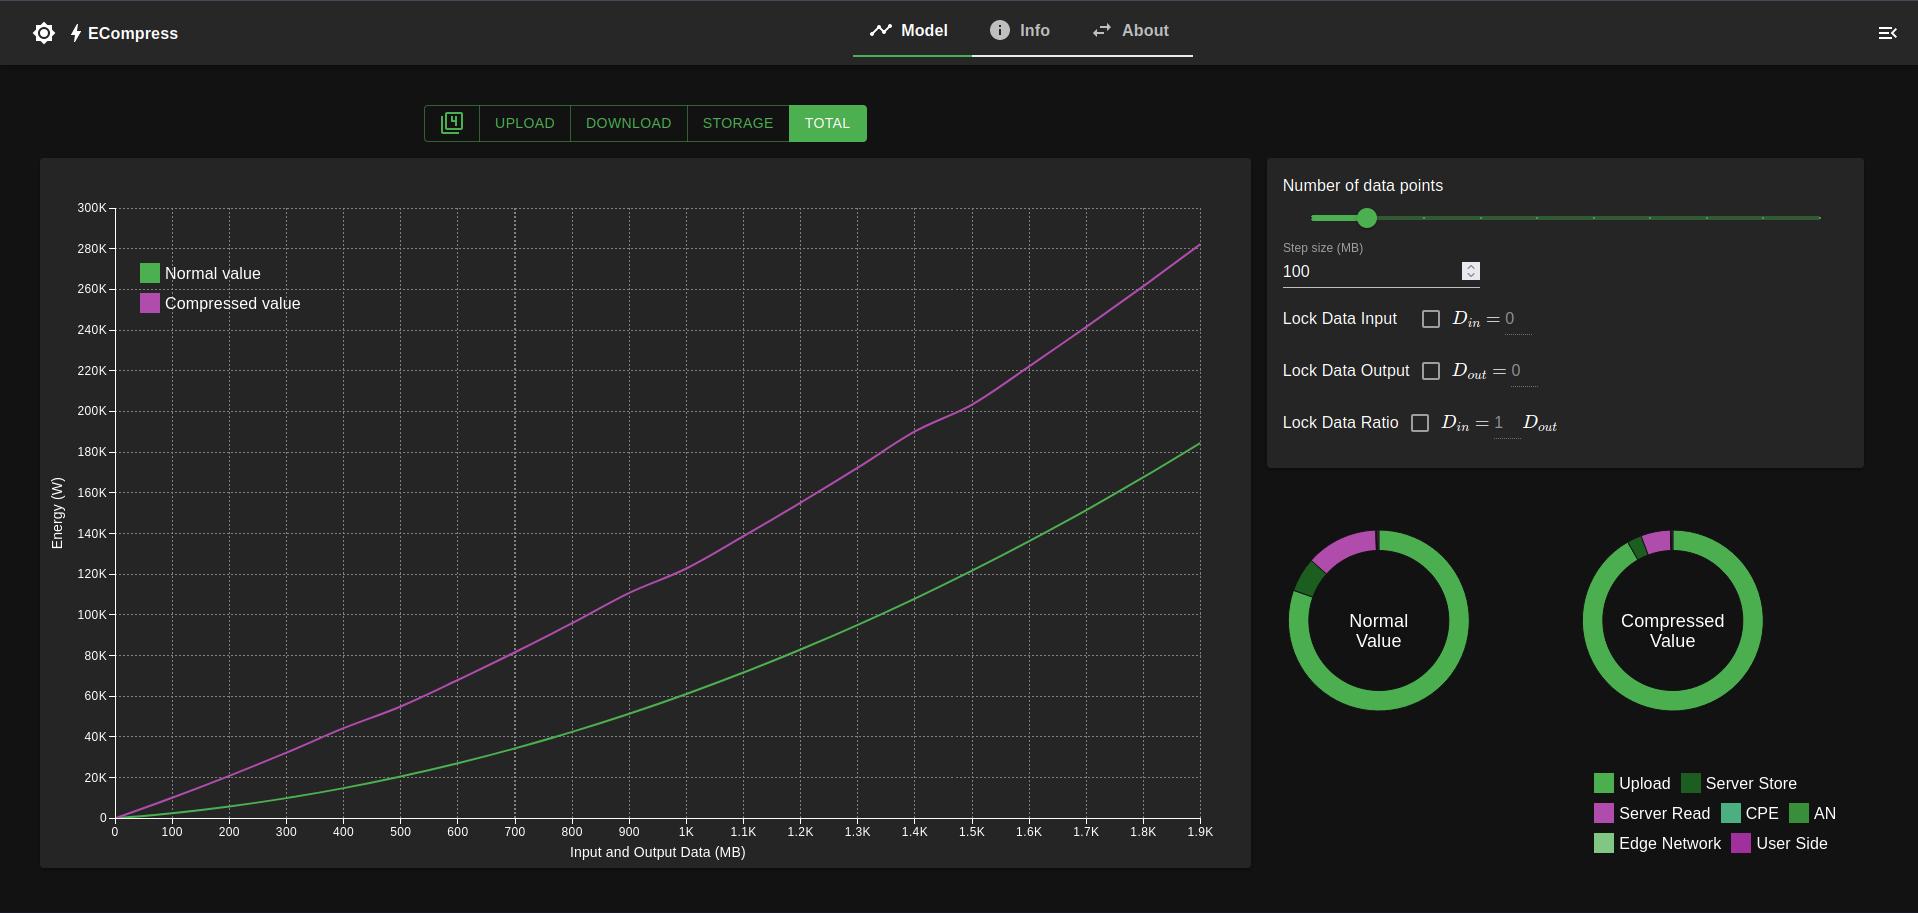
\includegraphics[width=1\textwidth]{figs/web_model_page_close.png}
            \caption{Model page of the Ecompress website.}
            \label{fig:web_model_page}
        \end{figure}

        The user can select one of 5 different visualization modes. It can be the whole energy model described in the previous chapter (chapter \ref{chapter:energy_model}), or any of the three sub-models that form the whole model, as well, as the option to show all the four models together. 

        The line chart, Figure \ref{fig:web_model_linechart}, shows two plots, one for the normal data and one for the chosen compression algorithm. The x-axis represents the size of data passing through the system, while the y-axis represents the energy consumption. In the case of the whole model, because there exists a difference between the input data (used by the upload and storage model) and the output data (used by the download model), the x-axis represents the size of both the input and output data (not cumulative). The user can select to lock one of the data types to a specific value, turning the x-axis into the variation of the other data type, or they can input a ratio between the two data types, which will split the x-axis into top and bottom, representing the output and input data sizes, respectively.
        
        \begin{figure}[H]
            \centering
            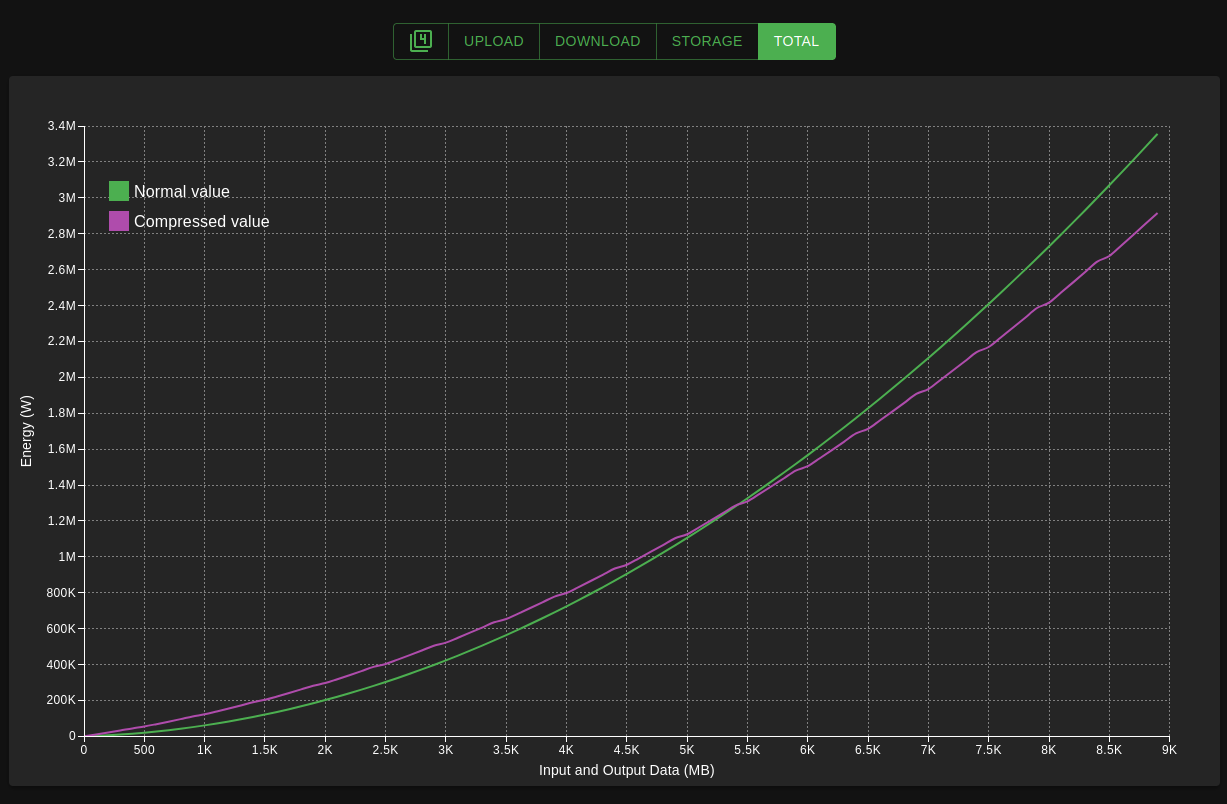
\includegraphics[width=0.8\textwidth]{figs/web_model_linechart.png}
            \caption[Line chart of the Ecompress website.] {Line chart of the Ecompress website. The green line represents the normal energy consumption, while the purple line represents the energy consumption when using a compression algorithm. On top, it shows a group of buttons to select the sub-model to be displayed.}
            \label{fig:web_model_linechart}
        \end{figure}
        
        Furthermore, the user can select any that point which will show two pie plots that show the contribution of each system component to the total energy consumption, for both the normal and compressed data. This is shown in Figure \ref{fig:web_model_piechart}.

        \begin{figure}[H]
            \centering
            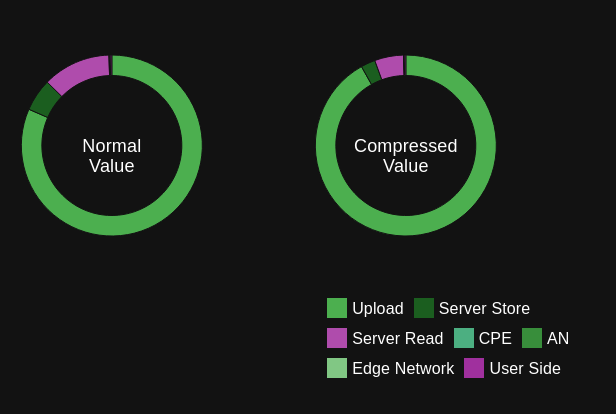
\includegraphics[width=0.6\textwidth]{figs/web_model_piechart.png}
            \caption[Pie chart of the Ecompress website.] {Pie chart of the Ecompress website. The left pie represents the normal energy consumption, while the right pie represents the energy consumption when using a compression algorithm.}
            \label{fig:web_model_piechart}
        \end{figure}

        It is also provided the ability to select the number of data points to be generated, as well as the time interval between each data point.

        To change the parameters, the user can click on the drawer open button, which will change the layout of the page to show side by side the graph and the form, as shown in Figure \ref{fig:web_calculator_drawer_open}. To return to the previous view, the user can click the same button, which will close the drawer.

        \begin{figure}[H]
            \centering
            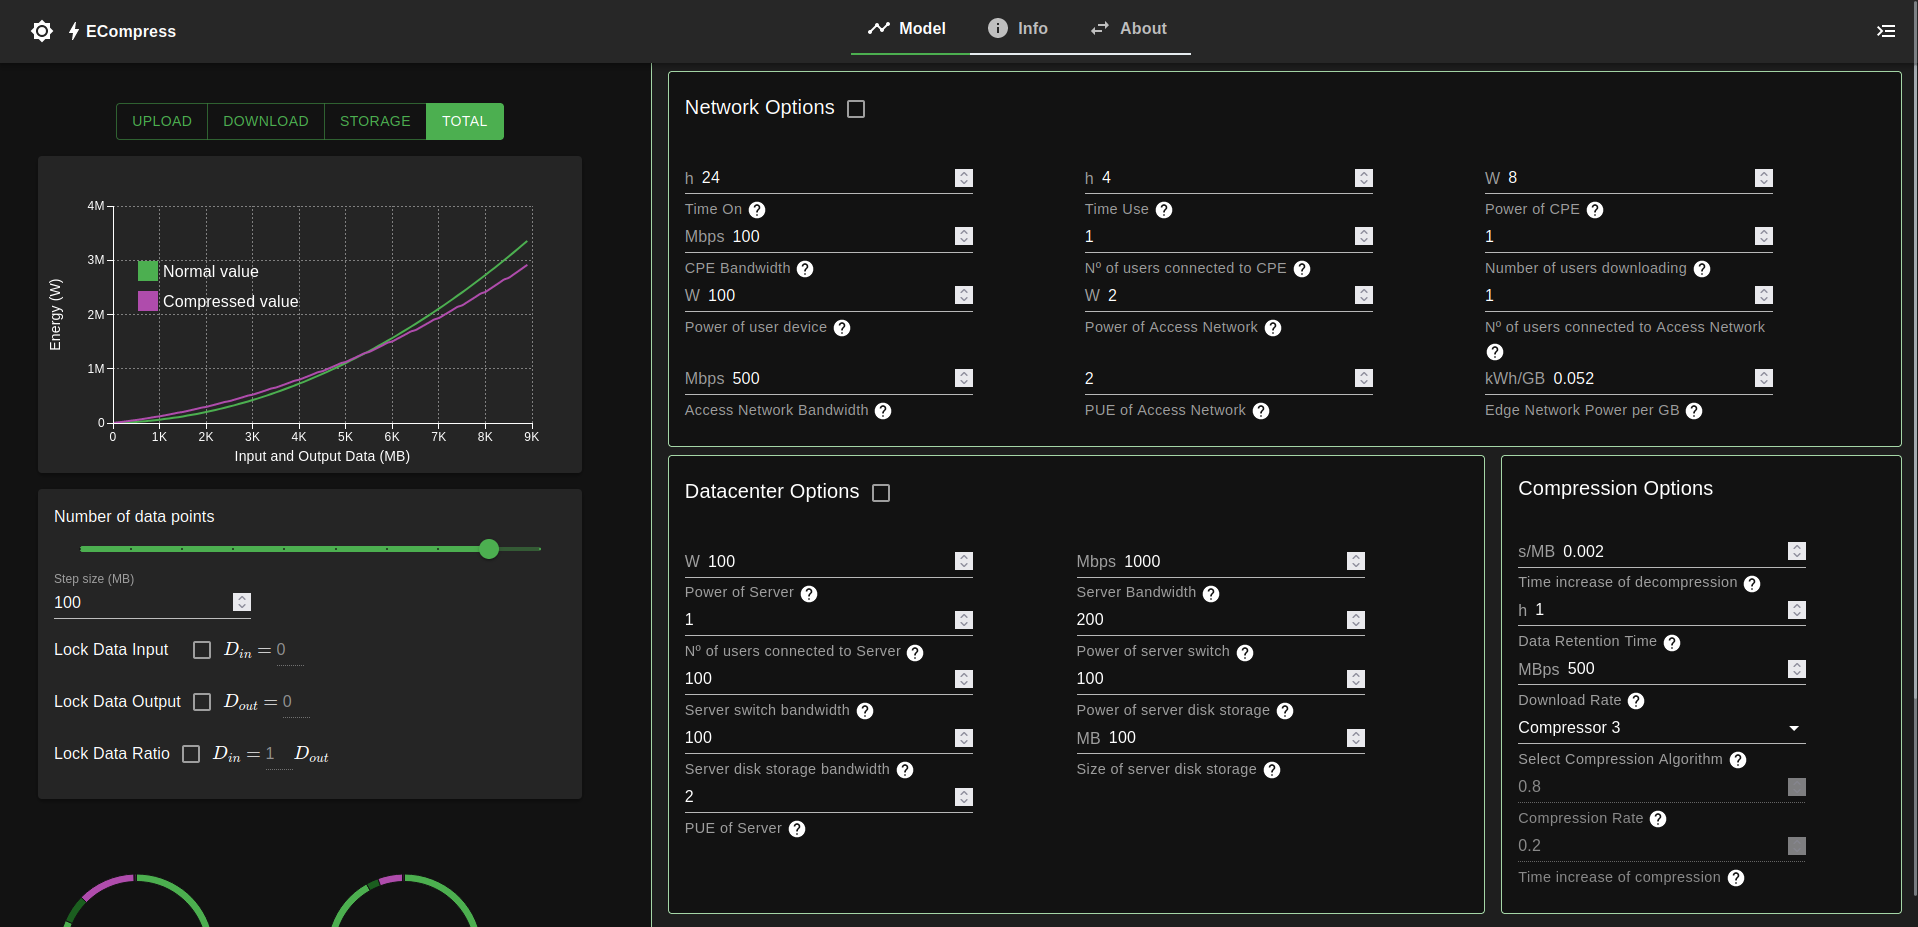
\includegraphics[width=1\textwidth]{figs/web_model_page_open.png}
            \caption[Model page of the Ecompress website with the drawer open.]{Model page of the Ecompress website with the drawer open. The contents of the graph are moved to the right, occupying one third of the screen, while the form is shown on the left, occupying two thirds of the screen.}
            \label{fig:web_calculator_drawer_open}
        \end{figure}

        The form is divided by each system component, and the user needs to submit with valid inputs for the data generation to start. The website doesn't provide an account option to save the user's preferences, however local storage is used to save the last parameters used by the user. 

    \subsubsection{Info page}

        The Info page (figure \ref{fig:info_page}) is a simple documentation page that explains how the energy models work, exposing the mathematical equations behind each graph.

        \begin{figure}[H]
            \centering
            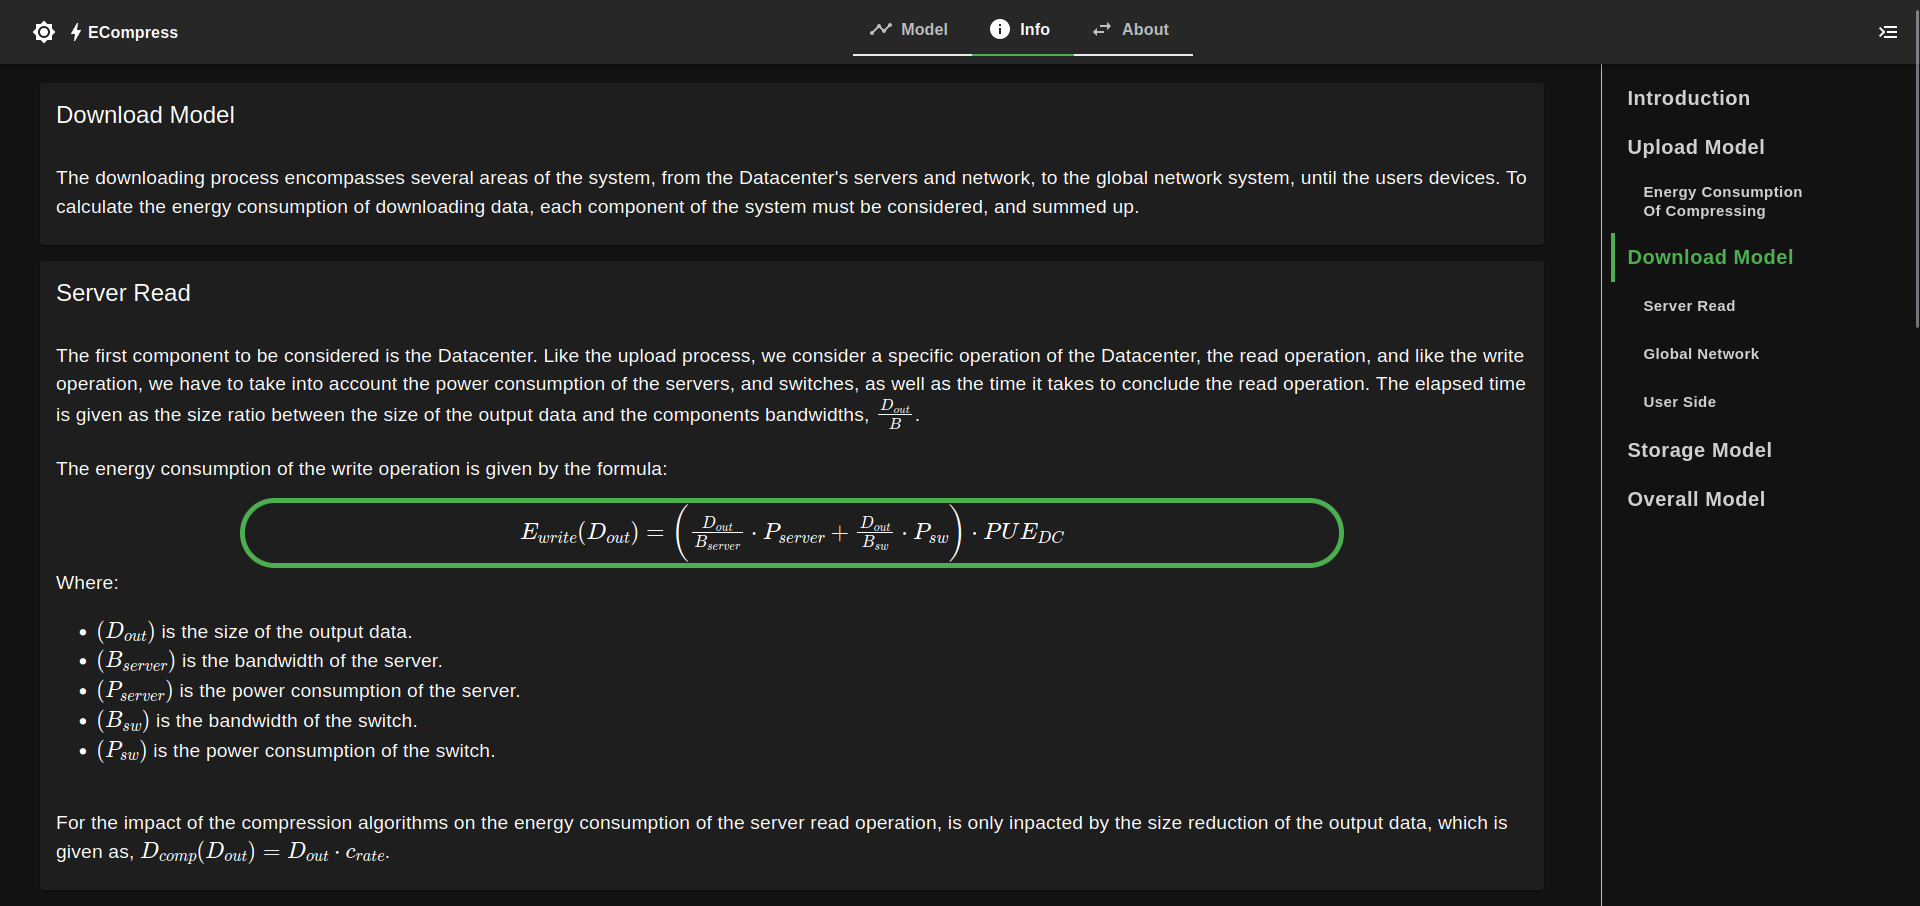
\includegraphics[width=1\textwidth]{figs/web_info_page.png}
            \caption{Information page of the Ecompress website.}
            \label{fig:info_page}
        \end{figure}

        The page is divided into several sub-pages that can be navigated through the sidebar which like the model can be collapsed for a fuller view of the content.

    \subsubsection{About page}

        The About page (figure \ref{fig:about_page}) shows information about the project, the authors and the institution behind the project. 


\section{Conclusion}

    